\documentclass[ignorenonframetext,]{beamer}
\setbeamertemplate{caption}[numbered]
\setbeamertemplate{caption label separator}{: }
\setbeamercolor{caption name}{fg=normal text.fg}
\beamertemplatenavigationsymbolsempty
\usepackage{lmodern}
\usepackage{amssymb,amsmath}
\usepackage{ifxetex,ifluatex}
\usepackage{fixltx2e} % provides \textsubscript
\ifnum 0\ifxetex 1\fi\ifluatex 1\fi=0 % if pdftex
  \usepackage[T1]{fontenc}
  \usepackage[utf8]{inputenc}
\else % if luatex or xelatex
  \ifxetex
    \usepackage{mathspec}
  \else
    \usepackage{fontspec}
  \fi
  \defaultfontfeatures{Ligatures=TeX,Scale=MatchLowercase}
\fi
\usetheme[]{Singapore}
\usefonttheme{serif}
% use upquote if available, for straight quotes in verbatim environments
\IfFileExists{upquote.sty}{\usepackage{upquote}}{}
% use microtype if available
\IfFileExists{microtype.sty}{%
\usepackage{microtype}
\UseMicrotypeSet[protrusion]{basicmath} % disable protrusion for tt fonts
}{}
\newif\ifbibliography
\hypersetup{
            pdftitle={Module 1: INTRODUCTION},
            pdfauthor={Stefanie Muff, Department of Mathematical Sciences, NTNU},
            colorlinks=true,
            linkcolor=Maroon,
            citecolor=Blue,
            urlcolor=blue,
            breaklinks=true}
\urlstyle{same}  % don't use monospace font for urls
\usepackage{color}
\usepackage{fancyvrb}
\newcommand{\VerbBar}{|}
\newcommand{\VERB}{\Verb[commandchars=\\\{\}]}
\DefineVerbatimEnvironment{Highlighting}{Verbatim}{commandchars=\\\{\}}
% Add ',fontsize=\small' for more characters per line
\usepackage{framed}
\definecolor{shadecolor}{RGB}{248,248,248}
\newenvironment{Shaded}{\begin{snugshade}}{\end{snugshade}}
\newcommand{\KeywordTok}[1]{\textcolor[rgb]{0.13,0.29,0.53}{\textbf{#1}}}
\newcommand{\DataTypeTok}[1]{\textcolor[rgb]{0.13,0.29,0.53}{#1}}
\newcommand{\DecValTok}[1]{\textcolor[rgb]{0.00,0.00,0.81}{#1}}
\newcommand{\BaseNTok}[1]{\textcolor[rgb]{0.00,0.00,0.81}{#1}}
\newcommand{\FloatTok}[1]{\textcolor[rgb]{0.00,0.00,0.81}{#1}}
\newcommand{\ConstantTok}[1]{\textcolor[rgb]{0.00,0.00,0.00}{#1}}
\newcommand{\CharTok}[1]{\textcolor[rgb]{0.31,0.60,0.02}{#1}}
\newcommand{\SpecialCharTok}[1]{\textcolor[rgb]{0.00,0.00,0.00}{#1}}
\newcommand{\StringTok}[1]{\textcolor[rgb]{0.31,0.60,0.02}{#1}}
\newcommand{\VerbatimStringTok}[1]{\textcolor[rgb]{0.31,0.60,0.02}{#1}}
\newcommand{\SpecialStringTok}[1]{\textcolor[rgb]{0.31,0.60,0.02}{#1}}
\newcommand{\ImportTok}[1]{#1}
\newcommand{\CommentTok}[1]{\textcolor[rgb]{0.56,0.35,0.01}{\textit{#1}}}
\newcommand{\DocumentationTok}[1]{\textcolor[rgb]{0.56,0.35,0.01}{\textbf{\textit{#1}}}}
\newcommand{\AnnotationTok}[1]{\textcolor[rgb]{0.56,0.35,0.01}{\textbf{\textit{#1}}}}
\newcommand{\CommentVarTok}[1]{\textcolor[rgb]{0.56,0.35,0.01}{\textbf{\textit{#1}}}}
\newcommand{\OtherTok}[1]{\textcolor[rgb]{0.56,0.35,0.01}{#1}}
\newcommand{\FunctionTok}[1]{\textcolor[rgb]{0.00,0.00,0.00}{#1}}
\newcommand{\VariableTok}[1]{\textcolor[rgb]{0.00,0.00,0.00}{#1}}
\newcommand{\ControlFlowTok}[1]{\textcolor[rgb]{0.13,0.29,0.53}{\textbf{#1}}}
\newcommand{\OperatorTok}[1]{\textcolor[rgb]{0.81,0.36,0.00}{\textbf{#1}}}
\newcommand{\BuiltInTok}[1]{#1}
\newcommand{\ExtensionTok}[1]{#1}
\newcommand{\PreprocessorTok}[1]{\textcolor[rgb]{0.56,0.35,0.01}{\textit{#1}}}
\newcommand{\AttributeTok}[1]{\textcolor[rgb]{0.77,0.63,0.00}{#1}}
\newcommand{\RegionMarkerTok}[1]{#1}
\newcommand{\InformationTok}[1]{\textcolor[rgb]{0.56,0.35,0.01}{\textbf{\textit{#1}}}}
\newcommand{\WarningTok}[1]{\textcolor[rgb]{0.56,0.35,0.01}{\textbf{\textit{#1}}}}
\newcommand{\AlertTok}[1]{\textcolor[rgb]{0.94,0.16,0.16}{#1}}
\newcommand{\ErrorTok}[1]{\textcolor[rgb]{0.64,0.00,0.00}{\textbf{#1}}}
\newcommand{\NormalTok}[1]{#1}
\usepackage{graphicx,grffile}
\makeatletter
\def\maxwidth{\ifdim\Gin@nat@width>\linewidth\linewidth\else\Gin@nat@width\fi}
\def\maxheight{\ifdim\Gin@nat@height>\textheight0.8\textheight\else\Gin@nat@height\fi}
\makeatother
% Scale images if necessary, so that they will not overflow the page
% margins by default, and it is still possible to overwrite the defaults
% using explicit options in \includegraphics[width, height, ...]{}
\setkeys{Gin}{width=\maxwidth,height=\maxheight,keepaspectratio}

% Prevent slide breaks in the middle of a paragraph:
\widowpenalties 1 10000
\raggedbottom

\AtBeginPart{
  \let\insertpartnumber\relax
  \let\partname\relax
  \frame{\partpage}
}
\AtBeginSection{
  \ifbibliography
  \else
    \let\insertsectionnumber\relax
    \let\sectionname\relax
    \frame{\sectionpage}
  \fi
}
\AtBeginSubsection{
  \let\insertsubsectionnumber\relax
  \let\subsectionname\relax
  \frame{\subsectionpage}
}

\setlength{\parindent}{0pt}
\setlength{\parskip}{6pt plus 2pt minus 1pt}
\setlength{\emergencystretch}{3em}  % prevent overfull lines
\providecommand{\tightlist}{%
  \setlength{\itemsep}{0pt}\setlength{\parskip}{0pt}}
\setcounter{secnumdepth}{0}
\usepackage{xcolor}

\title{Module 1: INTRODUCTION}
\subtitle{TMA4268 Statistical Learning V2020}
\author{Stefanie Muff, Department of Mathematical Sciences, NTNU}
\date{January xx and yy, 2020}

\begin{document}
\frame{\titlepage}

\begin{frame}

\end{frame}

\begin{frame}{Introduction}

\begin{block}{Aims of the first module}

\begin{itemize}
\item
  What is statistical learning?
\item
  Types of problems we will look at
\item
  Course overview and learning outcome, activities and team
\item
  Course modules, practical details (Blackboard)
\item
  Getting to know you -- who are you? Background?
\item
  Key concepts from your first course in statistics -- that you will
  need now, mixed with notation for this course
\item
  Introduction to R and RStudio\\
\end{itemize}

\end{block}

\end{frame}

\begin{frame}

\begin{block}{Learning material for this module}

\begin{itemize}
\item
  Our textbook James et al (2013): An Introduction to Statistical
  Learning - with Applications in R (ISL). Chapter 1 and 2.3.
\item
  \href{https://www.math.ntnu.no/emner/TMA4268/2019v/1Intro/Rbeginner.html}{\texttt{Rbeginner}}
  and
  \href{https://www.math.ntnu.no/emner/TMA4268/2019v/1Intro/Rintermediate.html}{\texttt{Rintermediate}}
\item
  Link to background on Matrix Algebra:
  \href{https://link.springer.com/chapter/10.1007/978-3-662-45171-7_2}{Härdle
  and Simes (2015) - A short excursion into Matrix Algebra} (on the
  reading list for TMA4267 Linear statistical models).
\end{itemize}

\end{block}

\end{frame}

\begin{frame}{What is statistical learning?}

\begin{itemize}
\item
  Refers to \emph{a vast set of tools to understanding data} (text book,
  p.~1).
\item
  Focuses on the whole chain:
\end{itemize}

model \(\rightarrow\) method \(\rightarrow\) algorithm \(\rightarrow\)
analysis \(\rightarrow\) interpretation

\begin{itemize}
\item
  Both \textbf{prediction} and \textbf{understanding} (inference
  \(\rightarrow\) drawing conclusions).
\item
  Statistical learning is a statistical discipline.
\end{itemize}

\end{frame}

\begin{frame}{Statistical Learning vs. ``Machine Learning''}

Machine learning is more focused on the algorithmic part of learning,
and is a discipline in computer science.

But, many methods/algorithms are common to the fields of statistical
learning and machine learning.

\end{frame}

\begin{frame}{Statistical Learning vs. ``Data Science''}

In data science the aim is to

\begin{itemize}
\tightlist
\item
  extract knowledge and understanding from data, and
\item
  requires a combination of statistics, mathematics, numerics, computer
  science and informatics.
\end{itemize}

This encompasses the whole process of data acquisition/scraping, going
from unstructured to structured data, setting up a data model,
performing data analysis, implementing tools and interpreting results.

In statistical learning we will not work on the two first above
(scraping and unstructured to structured).

\href{http://r4ds.had.co.nz/}{R for Data Science} is an excellent read
and relevant for this course!

\end{frame}

\begin{frame}{Problems you will learn to solve}

There are \textbf{three main types of problems} discussed in this
course:

\begin{itemize}
\item
  Regression
\item
  Classification
\item
  Unsupervised methods
\end{itemize}

using data from science, technology, industry, economy/finance, \ldots{}

\end{frame}

\begin{frame}[fragile]{Example 1: Regression (Etiology of CVD)}

\begin{itemize}
\item
  The Framingham Heart Study investigates the underlying causes of
  cardiovascular disease (CVD) (see
  \url{https://www.framinghamheartstudy.org/}). 
\item
  Aim: modelling systolic blood pressure (\texttt{SYSBP}) using data
  from \(n=2600\) persons.
\item
  For each person in the data set we have measurements of the following
  seven variables.
\end{itemize}

\scriptsize

\begin{itemize}
\tightlist
\item
  \texttt{SYSBP} systolic blood pressure (mmHg),
\item
  \texttt{SEX} 1=male, 2=female,
\item
  \texttt{AGE} age (years),
\item
  \texttt{CURSMOKE} current cigarette smoking at examination: 0=not
  current smoker, 1= current smoker,
\item
  \texttt{BMI} body mass index,
\item
  \texttt{TOTCHOL} serum total cholesterol (mg/dl),
\item
  \texttt{BPMEDS} use of anti-hypertensive medication at examination:
  0=not currently using, 1=currently using. \normalsize
\end{itemize}

\end{frame}

\begin{frame}

\includegraphics{1Intro_files/figure-beamer/CVDread-1.pdf}

What does this plot show?

Red: male; turquoise: female

\end{frame}

\begin{frame}

\begin{itemize}
\tightlist
\item
  Diagonal: density plot (generalization of histogram), or barplot.
\item
  Lower diagonals: scatterplot, histograms
\item
  Upper diagonals: correlations values or boxplots
\end{itemize}

\end{frame}

\begin{frame}

\begin{block}{Etiology of CVD - model}

\begin{itemize}
\item
  A \emph{multiple normal linear regression model} was fitted to the
  data set with \[-\frac{1}{\sqrt{\texttt{SYSBP}}}\] as response
  (output) and all the other variables as covariates (inputs).
\item
  The results are used to formulate hypotheses about the etiology of CVD
  - to be studied in new trials.
\end{itemize}

\end{block}

\end{frame}

\begin{frame}[fragile]

\scriptsize

\begin{Shaded}
\begin{Highlighting}[]
\NormalTok{modelB =}\StringTok{ }\KeywordTok{lm}\NormalTok{(}\OperatorTok{-}\DecValTok{1}\OperatorTok{/}\KeywordTok{sqrt}\NormalTok{(SYSBP) }\OperatorTok{~}\StringTok{ }\NormalTok{SEX }\OperatorTok{+}\StringTok{ }\NormalTok{AGE }\OperatorTok{+}\StringTok{ }\NormalTok{CURSMOKE }\OperatorTok{+}\StringTok{ }\NormalTok{BMI }\OperatorTok{+}\StringTok{ }\NormalTok{TOTCHOL }\OperatorTok{+}\StringTok{ }\NormalTok{BPMEDS, }
    \DataTypeTok{data =}\NormalTok{ thisds)}
\KeywordTok{summary}\NormalTok{(modelB)}\OperatorTok{$}\NormalTok{coeff}
\KeywordTok{summary}\NormalTok{(modelB)}\OperatorTok{$}\NormalTok{r.squared}
\KeywordTok{summary}\NormalTok{(modelB)}\OperatorTok{$}\NormalTok{adj.r.squared}
\end{Highlighting}
\end{Shaded}

\begin{verbatim}
##                  Estimate   Std. Error     t value     Pr(>|t|)
## (Intercept) -1.105693e-01 1.341653e-03 -82.4127584 0.000000e+00
## SEX2        -2.989392e-04 2.390278e-04  -1.2506465 2.111763e-01
## AGE          2.378224e-04 1.433876e-05  16.5859862 8.461545e-59
## CURSMOKE1   -2.504484e-04 2.526939e-04  -0.9911136 3.217226e-01
## BMI          3.087163e-04 2.954941e-05  10.4474583 4.696093e-25
## TOTCHOL      9.288023e-06 2.602433e-06   3.5689773 3.648807e-04
## BPMEDS1      5.469077e-03 3.265474e-04  16.7481874 7.297814e-60
## [1] 0.2493538
## [1] 0.2476169
\end{verbatim}

\end{frame}

\begin{frame}[fragile]

\scriptsize

\begin{Shaded}
\begin{Highlighting}[]
\KeywordTok{summary}\NormalTok{(modelB)}
\end{Highlighting}
\end{Shaded}

\begin{verbatim}
## 
## Call:
## lm(formula = -1/sqrt(SYSBP) ~ SEX + AGE + CURSMOKE + BMI + TOTCHOL + 
##     BPMEDS, data = thisds)
## 
## Residuals:
##        Min         1Q     Median         3Q        Max 
## -0.0207366 -0.0039157 -0.0000304  0.0038293  0.0189747 
## 
## Coefficients:
##               Estimate Std. Error t value Pr(>|t|)    
## (Intercept) -1.106e-01  1.342e-03 -82.413  < 2e-16 ***
## SEX2        -2.989e-04  2.390e-04  -1.251 0.211176    
## AGE          2.378e-04  1.434e-05  16.586  < 2e-16 ***
## CURSMOKE1   -2.504e-04  2.527e-04  -0.991 0.321723    
## BMI          3.087e-04  2.955e-05  10.447  < 2e-16 ***
## TOTCHOL      9.288e-06  2.602e-06   3.569 0.000365 ***
## BPMEDS1      5.469e-03  3.265e-04  16.748  < 2e-16 ***
## ---
## Signif. codes:  0 '***' 0.001 '**' 0.01 '*' 0.05 '.' 0.1 ' ' 1
## 
## Residual standard error: 0.005819 on 2593 degrees of freedom
## Multiple R-squared:  0.2494, Adjusted R-squared:  0.2476 
## F-statistic: 143.6 on 6 and 2593 DF,  p-value: < 2.2e-16
\end{verbatim}

\normalsize

\end{frame}

\begin{frame}[fragile]{Example 2: Classification (iris plants)}

The \texttt{iris} flower data set is a very famous multivariate data set
introduced by the British statistician and biologist Ronald Fisher in
1936.

The data set contains \textbf{three plant species} \{setosa, virginica,
versicolor\} and \textbf{four features measured} for each corresponding
sample: \texttt{Sepal.Length}, \texttt{Sepal.Width},
\texttt{Petal.Length} and \texttt{Petal.Width}.

\end{frame}

\begin{frame}

\begin{figure}
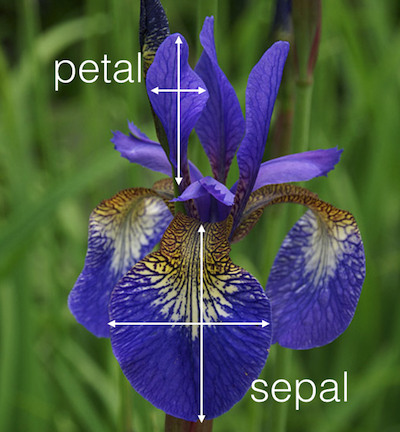
\includegraphics[width=150pt]{iris} \caption{Iris plant with sepal and petal leaves}\label{fig:iris_pic}
\end{figure}

\url{http://blog.kaggle.com/2015/04/22/scikit-learn-video-3-machine-learning-first-steps-with-the-iris-dataset/}

\end{frame}

\begin{frame}[fragile]

\scriptsize

\begin{Shaded}
\begin{Highlighting}[]
\KeywordTok{head}\NormalTok{(iris)}
\end{Highlighting}
\end{Shaded}

\begin{verbatim}
##   Sepal.Length Sepal.Width Petal.Length Petal.Width Species
## 1          5.1         3.5          1.4         0.2  setosa
## 2          4.9         3.0          1.4         0.2  setosa
## 3          4.7         3.2          1.3         0.2  setosa
## 4          4.6         3.1          1.5         0.2  setosa
## 5          5.0         3.6          1.4         0.2  setosa
## 6          5.4         3.9          1.7         0.4  setosa
\end{verbatim}

\normalsize

\end{frame}

\begin{frame}

Aim: correctly classify the species of an iris plant from sepal length
and sepal width.

\includegraphics{1Intro_files/figure-beamer/iriscont-1.pdf}

\end{frame}

\begin{frame}

\begin{block}{Linear boundaries}

In this plot the small black dots represent correctly classified iris
plants, while the red dots represent misclassifications. The big black
dots represent the class means.

~

\includegraphics[width=10cm]{1Intro_files/figure-beamer/irislda-1}

\end{block}

\end{frame}

\begin{frame}

\begin{block}{Non-linear boundaries}

Sometimes a more suitable boundary is not linear.\\
\hspace*{0.333em}

\includegraphics[width=10cm]{1Intro_files/figure-beamer/irisqda-1}

\end{block}

\end{frame}

\begin{frame}{Example 3: Unsupervised methods (Gene expression)}

\begin{itemize}
\tightlist
\item
  In a collaboration with researchers the Faculty of Medicine and Health
  the relationship between inborn maximal oxygen uptake and skeletal
  muscle gene expression was studied.
\item
  Rats were artificially selected for high- and low running capacity
  (HCR and LCR, respectively),
\item
  Rats were either kept seditary or trained.
\item
  Transcripts significantly related to running capacity and training
  were identified 
\item
  To further present the findings heat map of the most significant
  transcripts were presented (high expression are shown in red and
  transcripts with a low expression are shown in yellow).
\item
  This is hierarchical cluster analysis with pearson correlation
  distance measure.
\end{itemize}

\end{frame}

\begin{frame}

\begin{figure}
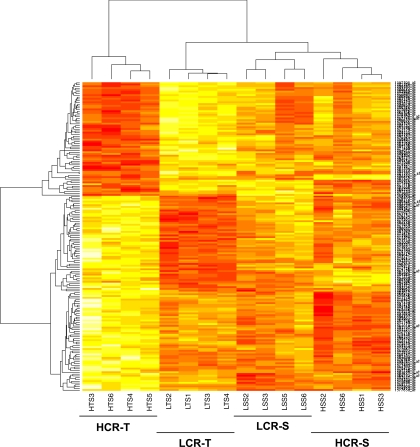
\includegraphics[width=150pt]{heatmap} \caption{Heatmap with dendrograms}\label{fig:heatmap_pic}
\end{figure}

More: \url{https://www.ncbi.nlm.nih.gov/pmc/articles/PMC2585023/}

\end{frame}

\begin{frame}{Who is this course for?}

\begin{block}{Primary requirements}

\begin{itemize}
\item
  Bachelor level: 3rd year student from Science or Technology programs,
  and master/PhD level students with interest in performing statistical
  analyses.
\item
  Statistics background: TMA4240/45 Statistics, ST1101+ST1201, or
  equivalent.
\item
  No background in statistical software needed: but we will use the R
  statistical software extensively in the course. Knowing python will
  make this easier for you!
\item
  Not a prerequisist but a good thing with knowledge of computing -
  preferably an introductory course in informatics, like TDT4105 or
  TDT4110.
\end{itemize}

\end{block}

\end{frame}

\begin{frame}

\begin{block}{Overlap}

\begin{itemize}
\item
  TDT4173 Machine learning and case based reasoning: courses differ in
  philosophy (computer science vs.~statistics). See Bb under FAQ for
  more details.
\item
  TMA4267 Linear Statistical Models: useful to know about multivariate
  random vectors, covariance matrices and the multivariate normal
  distribution. Overlap only for Multiple linear regression (M3).
\end{itemize}

\end{block}

\end{frame}

\begin{frame}{About the course}

\begin{block}{Focus: Statistical theory \textbf{and} doing analyses}

\begin{itemize}
\item
  The course has focus on \textbf{statistical theory}, but we apply all
  models and theory using (mostly) available function in R and real data
  sets.
\item
  It it important that the student in the end of the course \textbf{can
  analyse all types of data} (covered in the course) - not just
  understand the theory.
\item
  And vice versa - the student must also \textbf{understand} the model,
  methods and algorithms used.
\end{itemize}

\end{block}

\end{frame}

\begin{frame}

\begin{block}{Learning outcome}

\begin{enumerate}
\def\labelenumi{\arabic{enumi}.}
\item
  \textbf{Knowledge.} The student has knowledge about the most popular
  statistical learning models and methods that are used for
  \emph{prediction} and \emph{inference} in science and technology.
  Emphasis is on regression- and classification-type statistical models.
\item
  \textbf{Skills.} The student knows, based on an existing data set, how
  to choose a suitable statistical model, apply sound statistical
  methods, and perform the analyses using statistical software. The
  student knows how to present the results from the statistical
  analyses, and which conclusions can be drawn from the analyses.
\end{enumerate}

\end{block}

\end{frame}

\begin{frame}

\begin{block}{Course content}

Statistical learning, multiple linear regression, classification,
resampling methods, model selection/regularization, non-linearity,
support vector machines, tree-based methods, unsupervised methods,
neural nets.

\end{block}

\end{frame}

\begin{frame}

\begin{block}{Learning methods, activities and grading}

\begin{itemize}
\item
  Lectures, exercises and works (projects). ~
\item
  Portfolio assessment is the basis for the grade awarded in the course.
  This portfolio comprises

  \begin{itemize}
  \tightlist
  \item
    a written final examination (80\%).
  \item
    works (projects) (20\%). ~
  \end{itemize}
\item
  The results for the constituent parts are to be given in \%-points,
  while the grade for the whole portfolio (course grade) is given by the
  letter grading system. Retake of examination may be given as an oral
  examination. The lectures may be given in English.
\end{itemize}

\end{block}

\end{frame}

\begin{frame}

\begin{block}{Literature for the course}

~\\
\hspace*{0.333em}

\textbf{Textbook:} James, Witten, Hastie, Tibshirani (2013): ``An
Introduction to Statistical Learning''.

~\\
\textbf{Tentative reading list:} the whole book + the module pages+ two
compulsory exercises.

\end{block}

\end{frame}

\begin{frame}

\begin{block}{Course team}

~

\textbf{Lecturers:}

\begin{itemize}
\tightlist
\item
  Stefanie Muff (IMF/NTNU)
\item
  Thiago G. Martins (AIAscience and IMF/NTNU)?
\item
  Andreas Strand (NTNU)?
\end{itemize}

\textbf{Teaching assistents (TA)}

\begin{itemize}
\tightlist
\item
  Andreas Strand (head TA)?
\item
  Michail Spitieris?
\end{itemize}

\end{block}

\end{frame}

\begin{frame}{Teaching philosophy}

\begin{block}{The modules}

~

\begin{itemize}
\item
  Divide the topics of the course into modular units with specific
  focus.
\item
  This (hopefully) facilitates learning?
\item
  12 modules (weeks of teaching) =

  \begin{itemize}
  \tightlist
  \item
    introduction (this module)
  \item
    the 10 topics listed previously
  \item
    summing up\\
    \hspace*{0.333em}
  \end{itemize}
\item
  Two weeks without lectures (but supervision of exercises)
\end{itemize}

\end{block}

\end{frame}

\begin{frame}

\begin{block}{The lectures}

~

\textbf{Mondays at 8.15-10 in S4 and Thursdays at 14.15-16.00 in F6 or
Smia} ~

\begin{itemize}
\tightlist
\item
  We have \(2\cdot 2\) hours of lectures every week (except when working
  with the compulsory exercises).
\item
  Each week is a new topic and a new module
\item
  Some weeks (modules 2,5,7 and 9) the second lecture is an
  \emph{interactive lecture} in Smia, where active learning is in focus
  (more below).
\item
  The other weeks (modules 3,4,6,8,10 and 11) the second lecture is a
  plenary lecture in F6.
\item
  The first week of the course the second lecture is replaced by an R
  workshop!
\end{itemize}

\end{block}

\end{frame}

\begin{frame}

\begin{block}{The weekly supervision sessions}

~

\textbf{Thursdays 16.15-18 in Smia} ~\\
\hspace*{0.333em}

For each module \emph{recommended exercises} are given. These are partly

\begin{itemize}
\tightlist
\item
  theoretical exercises (from book or not)
\item
  computational tasks
\item
  data analysis
\end{itemize}

These are supervised in the weekly exercise slots.

We have joint supervision sessions with the TMA4267 Linear statistical
models course.

TAs from both courses will be present.

\end{block}

\end{frame}

\begin{frame}

\begin{block}{The compulsory exercises}

\begin{itemize}
\tightlist
\item
  There will be \textbf{two compulsory exercises}, each gives a maximal
  score of 15 points.
\item
  These are supervised in the weekly exercise slots and there will be
  one week without lectures (only with supervision) for each compulsory
  exercise.
\item
  Focus is both on theory and analysis and interpretation in R.
\item
  Students can work in groups (max size 3) and work must be handed in on
  Blackboard and be written in R Markdown (both .Rmd and .pdf handed
  in).
\item
  The TAs grade the exercises.
\item
  This gives 30\% of the final evaluation in the course, and the written
  exam the final 70\%.
\end{itemize}

\end{block}

\end{frame}

\begin{frame}

\begin{block}{How to use the module pages?}

\begin{itemize}
\tightlist
\item
  A slides version (output: beamer\_presentation) of the pages used in
  the plenary lectures.
\item
  A webpage version (output: html\_document) used in the interactive
  lectures.
\item
  A document version (output: pdf\_document) used for student self
  study.
\item
  The Rmd version - used as notebook to investigate changes to the R
  code.
\item
  Additional class notes (written in class) linked in.
\end{itemize}

The module pages are the backbone of the course!

\end{block}

\end{frame}

\begin{frame}{Student active learning}

We (probably) all have different ways in which we learn - and we have
different learning ambitions when attending a course.

~

\begin{block}{Felder and Silverman learning styles}

Back in 1988 Felder and Silverman published an article where they
suggested that there was a mismatch between the way students learn and
the way university courses were taught. They devised a taxonomy for
learning styles - where four different axis are defined:

\end{block}

\end{frame}

\begin{frame}

\begin{enumerate}
\def\labelenumi{\arabic{enumi})}
\tightlist
\item
  active - reflective: How do you process information: actively (through
  physical activities and discussions), or reflexively (through
  introspection)?
\item
  sensing-intuitive: What kind of information do you tend to receive:
  sensitive (external agents like places, sounds, physical sensation) or
  intuitive (internal agents like possibilities, ideas, through
  hunches)?
\item
  visual-verbal: Through which sensorial channels do you tend to receive
  information more effectively: visual (images, diagrams, graphics), or
  verbal (spoken words, sound)?
\item
  sequential - global: How do you make progress: sequentially (with
  continuous steps), or globally (through leaps and an integral
  approach)?
\end{enumerate}

\end{frame}

\begin{frame}

\begin{block}{The idea:}

\begin{itemize}
\item
  Acknowledging these different learning style axes
\item
  Choose teaching styles that matche the learning styles of the
  students.
\item
  Many students (according to Felder and coauthors) have a visual way of
  learning, and then teachers should spend time devising visual aids (in
  addition to verbal aids - that were the prominent aids in 1988), and
  so on.
\end{itemize}

\end{block}

\end{frame}

\begin{frame}

\begin{block}{Student active learning in TMA4268}

\begin{itemize}
\item
  Students have different background knowledge, learning ambitions and
  learning styles (verbal/visual, active/reflective, global/sequential,
  \ldots{}). ~
\item
  Teachers aim to make diverse learning resources available in courses,
  and ~
\item
  \emph{promote student active teaching methods}.
\end{itemize}

~

\textbf{Hypothesis:} Students will learn better/deeper with a
combination of different teaching methods.

\end{block}

\end{frame}

\begin{frame}

Therefore we aim to:

\begin{itemize}
\tightlist
\item
  Provide learning environments, opportunities, interactions, tasks and
  instruction that foster deep learning.
\item
  Provide guidance and support that challenges students based on their
  current ability.
\item
  Students discover their current strengths and weaknesses and what they
  need to do to improve.
\end{itemize}

We will now focus on \emph{active} and \emph{reflective} learning styles
and learning methods.

\end{frame}

\begin{frame}

\begin{block}{Active vs.~reflective learning styles}

\begin{block}{What are student reflective learning methods/tasks?}

\begin{itemize}
\tightlist
\item
  Plenary lectures
\item
  Reading textbook
\item
  Self study
\end{itemize}

\end{block}

\end{block}

\end{frame}

\begin{frame}

\begin{block}{Plenary lecture}

\begin{enumerate}
\def\labelenumi{\arabic{enumi})}
\tightlist
\item
  The teacher is lecturer
\item
  Limited amount of interaction student-lecturer
\item
  Limited amount of interaction student-student
\item
  Lecturer active, student passive
\item
  Where: lecture theatre, auditorium
\item
  Resources: (black)board, screen (for projector), microphone for
  lecturer, desks in rows.
\end{enumerate}

~

\textbf{Positive}: By using the traditional lecture method, lecturers
can present a large amount of material in a relatively brief amount of
time.

\textbf{Negative}: is it also efficient for the student? Maybe efficient
for students with a \emph{reflective learning style}?

\end{block}

\end{frame}

\begin{frame}

\begin{block}{What are student active learing methods/tasks?}

\begin{itemize}
\tightlist
\item
  Pause in plenary lecture to ask questions and let students think
  and/or discuss.
\item
  In-class quizzes (with the NTNU invention Kahoot!) - individual and
  team mode.
\item
  Projects - individual or in groups.
\item
  Group discussion
\item
  Interactive lectures
\end{itemize}

\end{block}

\end{frame}

\begin{frame}

\begin{block}{Interactive lecture}

\begin{enumerate}
\def\labelenumi{\arabic{enumi})}
\tightlist
\item
  The teacher is not a lecturer, but an advisor, and teaching assistent
  (TA) may also be present
\item
  Focus on interaction student-teacher
\item
  Focus on interaction student-student
\item
  Student and teacher/TA both active
\item
  Where: a room designed for interaction, collaboration and activity
\item
  Resources: (white)boards, screens, group tables, laptop/PC, possibly a
  podium for short announcements
\end{enumerate}

Positive: Studens are active. This is how work is done in many
cooperative environments (your future workplace?).

Negative: Challenging group processes. Unfamiliar setting for students?

Challenge: requires dedicated space and suitable problems to work on in
groups

\end{block}

\end{frame}

\begin{frame}

\begin{block}{Innovative learning space: Smia}

A room where interaction and activity is in focus. Flat floor with group
tables, whiteboard and screen - PC and electricity outlets.

~

\url{https://www.ntnu.no/laeringsarealer/smia}

\end{block}

\end{frame}

\begin{frame}

\begin{block}{Interactive lectures in Smia}

(modules 2,5,7 and 9): Work alone,in pairs, or larger groups (lecturer
help to form), introduction (5 min) - work on problem sets (35+,
lecturer and TA supervise) - summing up (5 min), pause, repeat. Lecturer
interrupts if common confusions or interesting observations by some of
the tables.

\end{block}

\end{frame}

\begin{frame}{The course modules}

(PL=plenary lecture in S4 (Mondays) or F6 (Thursdays), IL=interactive
lecture in Smia, E=exercise in Smia)

A detailed overview is found on Bb, and outside Bb in this
\href{https://www.math.ntnu.no/emner/TMA4268/2019v/table2019.html}{table}.

\begin{block}{1. Introduction}

{[}Ch 1, ML{]} 2019-w2 (PL: 07.01, R-workshop (IL/E): 10.01)

\begin{itemize}
\tightlist
\item
  About the course
\item
  Key concepts in statistics.
\item
  Intro to R and RStudio
\end{itemize}

\end{block}

\end{frame}

\begin{frame}

\begin{block}{2. Statistical Learning}

{[}Ch 2, ML{]} 2019-w3 (PL: 14.01, IL: 17.01 and E: 17.01)

\begin{itemize}
\tightlist
\item
  Estimating \(f\) (regression, classification), prediction accuracy vs
  model interpretability.
\item
  Supervised vs.~unsupervised learning
\item
  Bias-variance trade-off
\item
  The Bayes classifier and the KNN - a flexible method for regression
  and classification
\end{itemize}

First hours of IL: bias-variance trade off. Second hour: we target
students that doesn't plan to take TMA4267 Linear statistical models,
and we work with random vectors, covariance matrices and the
multivariate normal distribution (very useful before Modules 3 and 4).

\end{block}

\end{frame}

\begin{frame}

\begin{block}{3. Linear Regression}

{[}Ch 3, ML{]} 2019-w4 (PL: 21.01, PL: 24.01 and E: 24.01)

\begin{itemize}
\tightlist
\item
  Simple and multiple linear regression: model assumptions and data sets
\item
  Inference: Parameter estimation, CI, hypotheses, model fit
\item
  Coding of qualitative predictors
\item
  Problems and extensions
\item
  Linear regression vs.~KNN.
\end{itemize}

\end{block}

\begin{block}{4. Classification}

{[}Ch 4, ML{]} 2019-w5 (PL: 28.01, PL: 31.01 and E: 31.01)

\begin{itemize}
\tightlist
\item
  When to use classification (and not regression)?
\item
  Logistic regression
\item
  Linear discriminant analysis LDA and quadratic discriminant analysis
  QDA
\item
  Comparison of classificators
\end{itemize}

\end{block}

\end{frame}

\begin{frame}

\begin{block}{5. Resampling methods}

{[}Ch 5, ML{]} 2019-w7 (PL: 04.02, IL: 07.02, E: 07.02)

Two of the most commonly used resampling methods are cross-validation
and the bootstrap. Cross-validation is often used to choose appropriate
values for tuning parameters. Bootstrap is often used to provide a
measure of accuracy of a parameter estimate.

\begin{itemize}
\tightlist
\item
  Training, validation and test sets
\item
  Cross-validation
\item
  The bootstrap
\end{itemize}

\end{block}

\end{frame}

\begin{frame}

\begin{block}{Part 1: Modules 2-5}

is finished with compulsory exercise 1. In week 7 we have supervision in
Smia 11.02 (8.15-10.00), 14.02 (14.15-18.00).

To be decided: deadline for handing in Compulsory Ex 1. Suggestion:
Friday 22.02 at 16?

\end{block}

\end{frame}

\begin{frame}

\begin{block}{6. Linear Model Selection and Regularization}

{[}Ch 6, TGM{]} 2019-w8 (PL: 18.02, PL: 21.02, E: 21.02)

\begin{itemize}
\tightlist
\item
  Subset selection
\item
  Shrinkage methods (ridge and lasso)
\item
  Dimension reduction with principal components
\item
  Issues when working in high dimensions
\end{itemize}

\end{block}

\end{frame}

\begin{frame}

\begin{block}{7. Moving Beyond Linearity}

{[}Ch 7, AS/ML{]} 2019-w9 (PL: 25.02, IL: 28.02, E: 28.02 )

\begin{itemize}
\tightlist
\item
  Polynomial regression
\item
  Step functions
\item
  Basis functions
\item
  Regression and smoothing splines
\item
  Local regression
\item
  Generalized additive models
\end{itemize}

\end{block}

\end{frame}

\begin{frame}

\begin{block}{8. Tree-Based Methods}

{[}Ch 8, ML/TR{]} 2019-w10 (PL: 04.03, PL: 07.03, E: 07.03)

\begin{itemize}
\tightlist
\item
  Classification and regression trees
\item
  Trees vs linear models
\item
  Bagging, boosting and random forests
\end{itemize}

\end{block}

\begin{block}{9. Support Vector Machines}

{[}Ch9, ML{]} 2019-w11 (PL: 11.03, IL: 14.03, E: 14.03)

\begin{itemize}
\tightlist
\item
  Maximal margin classifiers
\item
  Support vector classifiers
\item
  Support vector machines
\item
  Two vs.~many classes
\item
  SVM vs.~logistic regression
\end{itemize}

\end{block}

\end{frame}

\begin{frame}

\begin{block}{10. Unsupervised learning}

{[}Ch 10, TGM{]} 2019-w12 (PL: 18.03, PL: 21.03, E:21.03)

\begin{itemize}
\tightlist
\item
  Principal component analysis
\item
  Clustering methods
\end{itemize}

\end{block}

\begin{block}{11. Neural Networks}

{[}ML{]} (PL: 25.03, PL: 28.03, E: 28.03)

\begin{itemize}
\tightlist
\item
  Network design and connections to previous methods
\item
  Fitting neural networks
\item
  Issues in training neural networks
\end{itemize}

\end{block}

\end{frame}

\begin{frame}

\begin{block}{Part 2: Modules 6-11}

is finished with compulsory exercise 2. In week 14 we have supervision
in Smia 01.04 (8.15-10.00), 04.04 (14.15-18.00).

To be decided: deadline for handing in Compulsory Ex 2. Suggestion:
Friday 12.04 at 16?

\end{block}

\begin{block}{12. Summing up and exam preparation}

{[}ML{]} 2019-w15 (PL: 08.04, E:11.04)

\begin{itemize}
\tightlist
\item
  Overview - common connections
\item
  Exam and exam preparation.
\end{itemize}

\end{block}

\end{frame}

\begin{frame}{Who are you - the students?}

Todo: Find out about kahoot!!

~

In class - go to kahoot.it to answer these questions. Answers in class
added, with 51 respondents.

\begin{block}{Study programme}

\begin{itemize}
\tightlist
\item
  MTFYMA FysMat ( )
\item
  BMAT ( )
\item
  MSMNFNA Master in Mathematical Sciences ( )
\item
  Other ( )
\end{itemize}

\end{block}

\begin{block}{Study year}

\begin{itemize}
\tightlist
\item
  1 or 2 ( )
\item
  3 ( )
\item
  4 ( )
\item
  5, \textgreater{}5 or PhD ( )
\end{itemize}

\end{block}

\end{frame}

\begin{frame}

\begin{block}{Have you/will you take TMA4267 Linear Statistical Models?}

\begin{itemize}
\tightlist
\item
  Yes, previously= in 2019 or earlier ( )
\item
  Yes, now= in 2020 ( )
\item
  Yes, planned for 2021 or later ( )
\item
  Not planned ( )
\end{itemize}

\end{block}

\begin{block}{Do you know R?}

\begin{itemize}
\tightlist
\item
  No ( )
\item
  No, and I do not want to learn R ( )
\item
  Yes, but only the basics ( )
\item
  Yes, in depth ( )
\end{itemize}

\end{block}

\end{frame}

\begin{frame}

\begin{block}{Plenary lectures on Monday mornings at 8.15-10 - do you
plan to attend?}

\begin{itemize}
\tightlist
\item
  Yes ( )
\item
  No, this is too early ( )
\item
  No, since I rarely attend lectures. ( )
\item
  No, for some other reason ( )
\end{itemize}

\end{block}

\begin{block}{What do you think will be most fun in TMA4268?}

\begin{itemize}
\tightlist
\item
  Learning new statistical theory ( )
\item
  Trying out statistical theory in R ( )
\item
  Analysing data ( )
\item
  Learn new hot topics ( )
\end{itemize}

\end{block}

\end{frame}

\begin{frame}{Practical details}

\begin{itemize}
\tightlist
\item
  go to Blackboard
\end{itemize}

\href{https://ntnu.blackboard.com/webapps/blackboard/execute/modulepage/view?course_id=_7960_1\&cmp_tab_id=_40192_1\&mode=view}{Guest
access}

Course information-Course modules-R resources-Compulsory
exercises-Reading list and resources-Exam

\end{frame}

\begin{frame}{Reference group}

\textbf{At least 3 members, one from}

\begin{itemize}
\tightlist
\item
  IndMat year 3
\item
  Any programme year 4
\item
  Not IndMat
\end{itemize}

Volunteers?

\end{frame}

\begin{frame}{Key concepts (stats) and notation}

\begin{block}{Todo -- compare to hand-written notes by Mette
(M1L1notes.pdf)}

\end{block}

\end{frame}

\begin{frame}{Plan for this week: Workshop for R and RStudio}

\begin{block}{Thursday January 10 at 14.15-18.00 in Smia}

Say here what the plan is

\end{block}

\end{frame}

\begin{frame}

\begin{block}{!Please do this before Thursday!}

\begin{itemize}
\item
  Install R: \url{https://www.r-project.org/about.html}
\item
  Install Rstudio \url{https://www.rstudio.com/products/rstudio/}
\end{itemize}

If you need help on installing R and RStudio on you laptop computer,
contact \href{mailto:orakel@ntnu.no}{\nolinkurl{orakel@ntnu.no}}.

\end{block}

\end{frame}

\begin{frame}[fragile]

\begin{block}{R, Rstudio, CRAN and GitHub - and R Markdown}

\begin{enumerate}
\def\labelenumi{\arabic{enumi})}
\item
  What is R? \url{https://www.r-project.org/about.html}
\item
  What is RStudio? \url{https://www.rstudio.com/products/rstudio/}
\item
  What is CRAN? \url{https://cran.uib.no/}
\item
  What is GitHub and Bitbucket? Do we need GitHub or Bitbucket in our
  course? \url{https://www.youtube.com/watch?v=w3jLJU7DT5E} and
  \url{https://techcrunch.com/2012/07/14/what-exactly-is-github-anyway/}
\item
  What is R Markdown?
\end{enumerate}

1-minute introduction video:
\url{https://rmarkdown.rstudio.com/lesson-1.html}

Then, if more is needed also a chapter from the Data Science book:
\url{http://r4ds.had.co.nz/r-markdown.html}

We will use R Markdown for writing the Compulsory exercise reports in
our course.

\begin{enumerate}
\def\labelenumi{\arabic{enumi})}
\setcounter{enumi}{5}
\tightlist
\item
  What is \texttt{knitr}? \url{https://yihui.name/knitr/}
\end{enumerate}

\end{block}

\end{frame}

\begin{frame}

\begin{block}{A first look at R and R studio}

\begin{itemize}
\tightlist
\item
  \href{https://www.math.ntnu.no/emner/TMA4268/2019v/1Intro/Rbeginner.html}{Rbeginner.html}
\item
  \href{https://www.math.ntnu.no/emner/TMA4268/2019v/1Intro/Rbeginner.pdf}{Rbeginner.pdf}
\item
  \href{https://www.math.ntnu.no/emner/TMA4268/2019v/1Intro/Rbeginner.Rmd}{Rbeginner.Rmd}
\end{itemize}

\end{block}

\end{frame}

\begin{frame}

\begin{block}{A second look at R and probability distributions}

\begin{itemize}
\tightlist
\item
  \href{https://www.math.ntnu.no/emner/TMA4268/2019v/1Intro/Rintermediate.html}{Rintermediate.html}
\item
  \href{https://www.math.ntnu.no/emner/TMA4268/2019v/1Intro/Rintermediate.pdf}{Rintermediate.pdf}
\item
  \href{https://www.math.ntnu.no/emner/TMA4268/2019v/1Intro/Rintermediate.Rmd}{Rintermediate.Rmd}
\end{itemize}

To see solutions added to the files, add -sol to filename to get *
\href{https://www.math.ntnu.no/emner/TMA4268/2019v/1Intro/Rintermediate-sol.html}{Rintermediate-sol.html}

\end{block}

\begin{block}{And resources about plots}

\begin{itemize}
\tightlist
\item
  \href{https://www.math.ntnu.no/emner/TMA4268/2019v/1Intro/Rplots.html}{Rplots.html}
\item
  \href{https://www.math.ntnu.no/emner/TMA4268/2019v/1Intro/Rplots.pdf}{Rplots.pdf}
\item
  \href{https://www.math.ntnu.no/emner/TMA4268/2019v/1Intro/Rplots.Rmd}{Rplots.Rmd}
\end{itemize}

To see solutions added to the files, add -sol to filename to get *
\href{https://www.math.ntnu.no/emner/TMA4268/2019v/1Intro/Rplots-sol.html}{Rplots-sol.html}

\end{block}

\end{frame}

\begin{frame}

\begin{block}{R resources}

\begin{itemize}
\item
  P. Dalgaard: Introductory statistics with R, 2nd edition, Springer,
  which is also available freely to NTNU students as an ebook:
  \href{http://link.springer.com/book/10.1007\%2F978-0-387-79054-1}{Introductory
  Statistics with R}.
\item
  Grolemund and Hadwick (2017): ``R for Data Science'',
  \url{http://r4ds.had.co.nz}
\item
  Hadwick (2009): ``ggplot2: Elegant graphics for data analysis''
  textbook:
  \url{https://link.springer.com/book/10.1007\%2F978-0-387-98141-3}
\item
  \href{https://www.rstudio.com/resources/cheatsheets/}{Overview of
  cheat sheets from RStudio}
\item
  Looking for nice tutorials: try
  \href{https://www.r-bloggers.com/}{Rbloggers!}
\item
  Questions on R: ask the course staff, colleagues, and
  \href{https://stackoverflow.com/}{stackoverflow}.
\end{itemize}

\end{block}

\end{frame}

\begin{frame}[fragile]{R packages}

If you want to look at the .Rmd file and \texttt{knit} it, you need to
first install the following packages (only once).

\begin{Shaded}
\begin{Highlighting}[]
\KeywordTok{install.packages}\NormalTok{(}\StringTok{"ggplot2"}\NormalTok{)}
\KeywordTok{install.packages}\NormalTok{(}\StringTok{"klaR"}\NormalTok{)}
\KeywordTok{install.packages}\NormalTok{(}\StringTok{"GGally"}\NormalTok{)}
\end{Highlighting}
\end{Shaded}

\end{frame}

\begin{frame}{Acknowledgements}

Thanks to Julia Debik for contributing to this module page.

\end{frame}

\end{document}
